\documentclass[output=paper]{langscibook}
\ChapterDOI{10.5281/zenodo.4727663}
\author{Richard Forsyth\affiliation{}}%affiliation intentionally left blank
\title{Cascading collocations: Collocades as correlates of formulaic language}
\abstract{This chapter focuses on a technique for detecting, measuring and displaying traces of formulaic language. For this purpose, a suite of computational procedures has been developed in order to quantify the degree to which individual texts and text types incorporate inflexible sequences of words. This development is predicated on the assumption that, even if we have no precise definition of formulaic language, it is widely accepted that it is characterized by repetition of fixed sequences. The method involves compiling a \textit{formulexicon} from a corpus of two or more text types and then using coverage by elements of that \textit{formulexicon} as an index of the degree to which a text, possibly absent from the training corpus, is pervaded by formulaic sequences. The problem of deciding what lengths of $n$-grams are warranted by the data is dealt with by the simple expedient of binarizing coverage counts by $n$-grams of various lengths. Trials on a variety of text types show that this allows \textit{collocades} -- cascades of collocations, whose lengths are not pre-determined -- to emerge from the data. Here the term \textit{collocation} is used in its broader sense, as in ``collocations are co-occurrences of words'' \citep[14]{Gries2009}. Software in Python~3 that implements this approach is available online under a Creative Commons licence. Examples of applying these procedures to a number of corpora illustrate some of the uses of this approach.}

% \keywords{collocades, corpus-driven research, formulaic language, linguistic statistics, multi-word units, phraseology}

\IfFileExists{../localcommands.tex}{
  \addbibresource{../localbibliography.bib}
  % add all extra packages you need to load to this file

\usepackage{tabularx,multicol}
\usepackage{url}
\urlstyle{same}

\usepackage{listings}
\lstset{basicstyle=\ttfamily,tabsize=2,breaklines=true}

\usepackage{langsci-optional}
\usepackage{langsci-lgr}
\usepackage{langsci-gb4e}

\usepackage{todonotes}
\usepackage{siunitx}
\sisetup{group-digits=false}

\usepackage{langsci-lgr}

\usepackage[linguistics]{forest}
\usepackage{subcaption}
\usepackage{pgfplots, pgfplotstable}
\usepgfplotslibrary{colorbrewer}

  \newcommand*{\orcid}{}

\makeatletter
\let\thetitle\@title
\let\theauthor\@author
\makeatother

\newcommand{\togglepaper}[1][0]{
%   \bibliography{../localbibliography}
  \papernote{\scriptsize\normalfont
    \theauthor.
    \titleTemp.
    To appear in:
    Aleksandar Trklja \& Łukasz Grabowski.
    Formulaic language: Theories and methods.
    Berlin: Language Science Press. [preliminary page numbering]
  }
  \pagenumbering{roman}
  \setcounter{chapter}{#1}
  \addtocounter{chapter}{-1}
}

\newcommand{\researchquestion}[2]{\begin{itemize}\item[\bfseries #1]\bfseries #2\end{itemize}}


\DeclareNewSectionCommand
  [
    counterwithin = chapter,
    afterskip = 2.3ex plus .2ex,
    beforeskip = -3.5ex plus -1ex minus -.2ex,
    indent = 0pt,
    font = \usekomafont{section},
    level = 1,
    tocindent = 1.5em,
    toclevel = 1,
    tocnumwidth = 2.3em,
    tocstyle = section,
    style = section
  ]
  {appendixsection}

\DeclareNewSectionCommand
  [
    counterwithin = appendixsection,
    beforeskip=-10pt,
    afterskip=1sp,
    indent = 0pt,
    font = \usekomafont{subsection},
    level = 2,
    tocindent = 3.8em,
    toclevel = 2,
    tocnumwidth = 3.2em,
    tocstyle = section,
    style = section
  ]
  {appendixsubsection}
  
\renewcommand*\theappendixsection{\Alph{appendixsection}}
\renewcommand*{\appendixsectionformat}{\appendixname~\theappendixsection\autodot\enskip}
\renewcommand*{\appendixsectionmarkformat}{\appendixname~\theappendixsection\autodot\enskip}


\newcommand{\glossF}{\textsc{f}}
\newcommand{\glossM}{\textsc{m}}
\newcommand{\glossV}{\textsc{v}}
\newcommand{\glossN}{\textsc{n}}
\newcommand{\INSTR}{\INS}
\newcommand{\PRON}{\textsc{pron}}
\newcommand{\PREP}{\textsc{prep}}
\newcommand{\NOUN}{\textsc{noun}}
\newcommand{\PAST}{\textsc{past}}
\newcommand{\ADESS}{\textsc{adess}}
% \newcommand{\ADJ}{\textsc{adj}}
\newcommand{\CONJ}{\textsc{conj}}
\newcommand{\ESSIVE}{\textsc{essive}}
\newcommand{\GERUND}{\textsc{gerund}}
\newcommand{\NEUT}{\textsc{neut}}
% \newcommand{\NOM}{\textsc{nom}}
\newcommand{\NOUNPROPER}{\textsc{nounproper}}
\newcommand{\PART}{\textsc{part}}
\newcommand{\PRES}{\textsc{pres}}
\newcommand{\glossINF}{\textsc{inf}}
% \newcommand{\PL}{\textsc{pl}}
% \newcommand{\POSS}{\textsc{poss}}
\newcommand{\POSTP}{\textsc{postp}}
\newcommand{\PRT}{\textsc{prt}}
\newcommand{\MOD}{\textsc{mod}}
\newcommand{\NN}{\textsc{nn}}
% \newcommand{\PTCP}{\textsc{ptcp}}


\newcommand{\ESS}{\textsc{ess}}
\newcommand{\NUM}{\textsc{num}}

\newcommand{\glottocodes}[1]{}



  %% hyphenation points for line breaks
%% Normally, automatic hyphenation in LaTeX is very good
%% If a word is mis-hyphenated, add it to this file
%%
%% add information to TeX file before \begin{document} with:
%% %% hyphenation points for line breaks
%% Normally, automatic hyphenation in LaTeX is very good
%% If a word is mis-hyphenated, add it to this file
%%
%% add information to TeX file before \begin{document} with:
%% %% hyphenation points for line breaks
%% Normally, automatic hyphenation in LaTeX is very good
%% If a word is mis-hyphenated, add it to this file
%%
%% add information to TeX file before \begin{document} with:
%% \include{localhyphenation}
\hyphenation{
affri-ca-te
affri-ca-tes
analy-sis
}

\hyphenation{
affri-ca-te
affri-ca-tes
analy-sis
}

\hyphenation{
affri-ca-te
affri-ca-tes
analy-sis
}

  \togglepaper[1]%%chapternumber
}{}

% \shorttitlerunninghead{}
\begin{document}
\SetupAffiliations{output affiliation=false}
\lstset{frame=lines}
\maketitle

\section{Introduction}\label{sec:forsyth:1}

Many linguists have celebrated the ``unlimited creative potential'' of human language \citep[117]{Eggins1994}. Ron \citet{Carter2004} has argued that creativity is an all-pervasive feature of everyday language, a point also emphasized by Chomsky.

\begin{quote}
The normal use of language relies in an essential way on this unboundedness, on the fact that language contains devices for generating sentences of arbitrary complexity. Repetition of sentences is a rarity; innovation, in accordance with the grammar of the language, is the rule in ordinary day-by-day performance. \citep[118]{Chomsky1972}\hbox{}
\end{quote}

On the other hand, others have noted the ``deadly repetitiousness of language" \citep[570]{Bolinger1965}. This refers to the fact that speakers and writers tend to reuse chunks of language, perhaps with slight variation, a phenomenon dubbed by \citet{Sinclair1991} ``the idiom principle''. Presumably this reflects a natural tendency to save mental effort. As \citet{Halliday_that_2014} puts it, ``repeated patterns require less brain power both to produce and to understand.''

This apparent contradiction points to a dimension on which examples of language use can vary widely, from creative to routine. Research into \textit{formulaic language} is at least in part an attempt to explore this polarity. However, the term refers to a wide variety of linguistic phenomena. Essentially, formulaic language is a negative concept: we recognize it when the creative potential of ordinary language, celebrated by Carter, Chomsky, Eggins and others, appears to be partially or completely restricted. Such restriction can happen for diverse reasons, which helps to explain why no precise, agreed definition exists of what exactly constitutes formulaic language, although many researchers are actively engaged in studying its manifestations, such as idioms, clichés, legal boiler-plate and apparently prefabricated lexical bundles.

It should perhaps be noted that, in contexts such as second-language learning, the use of multi-word units is sometimes viewed in a positive manner, as a sign that the learner is gaining phraseological competence. For instance, \citet{GrangerBestgen2014} and \citet{Leńko-Szymańska2016} explore the use of statistics relating to multi-word units as potential indices of learner competence. In this case the ability to deploy word groupings is evidence that the learner can operate with higher-level chunks.

In any case, whether or not formulaic language is viewed pejoratively or as valuable, we do not have a widely accepted method of assessing just where on the polarity from creative to formulaic a given text or corpus lies. A major objective of the present chapter is therefore to describe a computable index of linguistic flexibility\slash inflexibility which could serve to indicate the degree to which a text or text type exhibits formulaic language. This problem, namely to what degree a particular kind of language is formulaic, is one of the key questions in the field \citep[4]{Wray2002}, and one that has not been answered in a comprehensive manner.

Strictly speaking, without a definition of our key term, it should not be possible to measure the extent to which a given text or speech is formulaic. Nevertheless, the present chapter sets out to describe, and apply, procedures that are designed to provide researchers with a quantitative index to associate with more impressionistic judgements; and to help identify sections within texts that can be further scrutinized as embodying mainly prefabricated segments. This development is predicated on the assumption that, even if we have no precise definition of formulaic language, it is widely accepted that it is characterized by repetition of fixed sequences.

In short, we don't know exactly what formulaic language is, and suspect that it has multiple causes, but we will attempt to measure it anyway. This attitude isn't quite as unscientific as it might seem. One can compare the situation in biology, for example, regarding the crucial concept of \textbf{biodiversity}. Assessing biodiversity at various locations and trying to estimate the biodiversity of planet earth is something that scientists and many lay people agree is a matter of grave importance, although there is no single method for measuring it. Nevertheless, different researchers have proposed, and refined, a number of ways of quantifying the diversity of life forms in various habitats, which, between them, have helped to advance knowledge in this area \citep{Magurran2004}; consequently we can do better than mere guesswork when assessing whether and where biodiversity is increasing or decreasing.

In the sphere of linguistics, many studies have explored the phenomenon of collocation in a general sense, and several techniques have been developed to seek examples in corpora, using a variety of terms such as multi-word units, lexical bundles and others (e.g., \citealt{ShimohataEtAl1999,ZhangEtAl2009, KilgarriffEtAl2012}). Moreover, programs exist that are generally available, for example kfNgram \citep{Fletcher2012} and Wordsmith Tools \citep{Scott2020}, which automate some aspects of the search for co-occurring linguistic units. These tools and techniques are primarily aimed, however, at throwing light on the linguistic behaviour of the speakers or writers of the texts in question. In other words, the multi-item units discovered are regarded as results in themselves. Some researchers also limit themselves to pre-specified grammatical functions, such as noun phrases (e.g. \citealt{Daille2003,ZhangEtAl2009}) and thus presuppose reliance on ancillary parsing or tagging software. For this reason they are difficult or impossible to adapt to the main purpose of the present approach, which is to quantify the pervasiveness of such multi-item units in various texts and\slash or text types.

The method described in this chapter involves compiling a \textit{formulexicon} from a corpus of two or more text types and then using coverage by elements of that \textit{formulexicon} as an index of the degree to which a text, possibly absent from the training corpus, is pervaded by formulaic sequences. The problem of deciding what lengths of $n$-grams are warranted by the data is dealt with by the simple expedient of binarizing coverage counts by $n$-grams of various lengths. Trials on a variety of text types show that this allows \textit{collocades} -- cascades of collocations, whose lengths are not pre-determined -- to emerge from the data. The extent to which a text is covered by such collocades can be quantified as an index of the degree to which that text is formulaic. Software in Python~3 that implements this approach is available online under a Creative Commons licence.\footnote{The formulib package can be found at \url{http://www.richardsandesforsyth.net/software.html}. Sample text files are also freely available under a Creative Commons licence.}

\section{The formulib suite}\label{sec:forsyth:2}

To illustrate this approach, a small test corpus, consisting of seven subcorpora, has been compiled, as briefly described in \tabref{tab:forsyth:1}.

\begin{table}
\caption{Test corpora\label{tab:forsyth:1}}
\begin{tabularx}{\textwidth}{lQ}
\lsptoprule
Short name & Description\\\midrule
BEER & Texts from the back labels of beer bottles\\
EW & Short stories by Edith Wharton (1862--1937)\\
FEWREPS & Postings on Hong Kong Tripadvisor travel forum (2016) with fewer than 2 replies\\
LEAFLET & Information leaflets of medicines\\
MANYREPS & Postings on Hong Kong Tripadvisor travel forum (2016) with more than 10 replies\\
SRES & United Nations Security Council resolutions (1999--2004)\\
WINE & Texts from the back labels of wine bottles\\
\lspbottomrule
\end{tabularx}
\end{table}

Basic details of the numbers and sizes of these text collections are described in \tabref{tab:forsyth:2}.

\begin{table}
\small
\caption{Sizes of text corpora\label{tab:forsyth:2}}
\begin{tabularx}{\textwidth}{lYYYYr}
\lsptoprule
Short name & Texts & Tokens & Smallest & Median & Longest\\
\midrule
BEER &  118 &  15781 &  56 &  129 &  314\\
EW &  44 &  365158 &  2271 &  8228 &  15682\\
FEWREPS &  213 &  14898 &  17 &  56 &  359\\
LEAFLET &  461 &  482373 &  180 &  946 &  5251\\
MANYREPS &  610 &  65494 &  17 &  80 &  1468\\
SRES &  275 &  248676 &  102 &  635 &  5452\\
WINE &  86 &  11474 &  57 &  125 &  296\\
\lspbottomrule
\end{tabularx}
\end{table}

In \tabref{tab:forsyth:2} text lengths are given in tokens, which are normally words, although numbers, i.e. strings of numerals, also count as tokens. It will be seen that many of these documents are individually very short. The Hong Kong Tripadvisor postings can be as small as 17 tokens in length. The above texts are all in English. The system has been used with other languages, including Chinese, and can be applied to any language than can be encoded in Unicode (UTF-8).

The suite of programs in Python~3 that constitute the formulib package and their functions are summarized in \tabref{tab:forsyth:3}.

\begin{table}
\small
\caption{Programs of formulib and their functions\label{tab:forsyth:3}}
\begin{tabularx}{\textwidth}{>{\ttfamily}lQ}
\lsptoprule
Program & Function\\
\midrule
outgrams & The main input of this program is a collection of text files, normally divided into more than one text category. It compiles the components of a \textit{formulexicon} by finding the most frequent n1-grams up to n2-grams in two or more categories of text files where n1 is 2 and n2 is 5 by default.\\
formulex & This program takes a collection of text files of more than one category, typically the same collection as input to outgrams, and applies the \textit{formulexicon} already generated to compute coverage by collocades for each file and thereby indicate the extent of formulaic language in it. The program also produces a list of collocades, multi-word units whose lengths are derived from the data rather than being specified in advance (as will be explained below).\\
taverns & This program (Textual Affinity Values Employing Repeated N-gram Sequences) computes coverage of two or more categories of document not only by the collocades generated from their own category but by those of the other categories as well, thus identifying highly typical and highly atypical texts in each class. It also functions as a classifier by using coverage by collocades from all categories, to indicate likely category membership. Usually its input will be a holdout sample of text files which were not used in generating the $n$-gram lists.\\
flicshow & This program produces a colour-coded FLiC list (Formulaic Language in Context) designed to show how the collocades are distributed in various texts. (See \sectref{sec:forsyth:5}.)\\
postflab & This program takes a secondary output of formulex, the collocade list, and applies a 1-dimensional similarity scaling procedure to them, so that related sequences can be plotted in a way that reveals their inter-relationships. (See \sectref{sec:forsyth:6}.)\\
\lspbottomrule
\end{tabularx}
\end{table}

\clearpage
\section{The trouble with $n$-grams}\label{sec:forsyth:3}

The initial program of this suite, outgrams, is relatively conventional. Its main output, referred to here as a \textit{formulexicon}, is a list of the N most frequent $n$-grams for each category of the input text files, with $N=80$ by default. A segment of its output for the SRES category, when the minimum and maximum $n$-grams lengths were specified as 3 to 6 (tokens), follows. The software allows punctuation to be ignored or preserved, and, independently, for upper case to be preserved or changed to lower case. In this and subsequent examples, the option of removing punctuation was chosen, and lower case was enforced. Among other things, this illustrates why $n$-gram lists, in and of themselves, are not particularly enlightening.\bigskip

\begin{lstlisting}[language=Python,basicstyle=\footnotesize\ttfamily]
# sres 154799 978607

1 (6, 175, 34, ('adopted', 'by', 'the', 'security', 'council', 'at'))
2 (6, 175, 30, ('by', 'the', 'security', 'council', 'at', 'its'))
3 (6, 153, 36, ('the', 'democratic', 'republic', 'of', 'the', 'congo'))
4 (6, 130, 33, ('the', 'charter', 'of', 'the', 'united', 'nations'))
5 (6, 121, 35, ('the', 'report', 'of', 'the', 'secretary', 'general'))
6 (6, 97, 28, ('of', 'the', 'charter', 'of', 'the', 'united'))
7 (6, 95, 36, ('decides', 'to', 'remain', 'actively', 'seized', 'of'))
8 (6, 93, 36, ('remain', 'actively', 'seized', 'of', 'the', 'matter'))
9 (6, 92, 32, ('to', 'remain', 'actively', 'seized', 'of', 'the'))
10 (6, 87, 34, ('report', 'of', 'the', 'secretary', 'general', 'of'))

[.... many lines omitted ....]

1 (3, 624, 21, ('the', 'secretary', 'general'))
2 (3, 579, 18, ('the', 'united', 'nations'))
3 (3, 520, 20, ('the', 'security', 'council')) 
4 (3, 319, 17, ('the', 'government', 'of'))
5 (3, 312, 13, ('of', 'the', 'united'))
6 (3, 245, 16, ('of', 'the', 'secretary'))
7 (3, 243, 20, ('secretary', 'general', 'to'))
8 (3, 237, 18, ('in', 'accordance', 'with'))
9 (3, 207, 21, ('the', 'implementation', 'of'))
10 (3, 202, 22, ('requests', 'the', 'secretary'))
\end{lstlisting}

Here we have the ten most frequent 6-grams and the ten most frequent 3-grams derived from the SRES subcorpus. The top line indicates that these $n$-grams are based on 154,799 tokens which amount to 978,607 characters. This is less than the size given in \tabref{tab:forsyth:3} because the full dataset has been split randomly into training and test sets, of 1117 and 690 text files respectively.

The first two 6-grams both occur 175 times in this corpus. The first is 34 characters in length, including blanks between tokens, and the second is 30 characters long. It seems a fair inference that they arise from a 7-gram, namely ``adopted by the security council at its'', but that is hardly obvious from the listing. Likewise, if we take items 7, 8 and 9 together, which occur 95, 93 and 92 times respectively, with a bit of background knowledge, we might arrive at the phrase ``decides to remain actively seized of the matter'', an 8-gram with which many of these Security Council resolutions sign off. However, this also is not immediately obvious from the listing (which is in fact designed more to be read by other programs than by people).

The point applies also with the shorter $n$-grams. The first three 3-grams (with the benefit of background knowledge) would seem to be natural units in their own right. But alongside them, we find ``secretary general to'' and ``requests the secretary'', which are fragments of longer phrases.

What this illustrates is that in a standard frequency list of fixed-size $n$-grams, such as those exemplified above, longer $n$-grams tend to appear in the form of multiple fragments. It requires tedious inspection, along with background knowledge, to identify appropriate lengths for the fragmented pieces of repetitive phrasings. It is desirable for the computer to provide more help in that identification process.

\section{From $n$-grams to collocades}\label{sec:forsyth:4}

The formulex program is designed for this purpose. The basic idea behind this program is very simple. The problem with $n$-gram lists is that they tend to contain multiple fragments of longer sequences, losing track of what might be considered the natural length of the sequences from which they are derived. So formulex tries to put them back together by going back over the original texts to find out exactly which passages are covered by the items in the frequent $n$-gram list. The key concept here is \textit{coverage}. The important point is that a text sequence is either covered or not: the number of $n$-grams that match a particular sequence of tokens doesn't matter, just whether any do or none.

To give an illustration of the covering process, suppose that you have gathered a corpus of political propaganda in which the phrase \textit{securing a better future for hardworking families} is repeated ad nauseam.

This could be regarded as a frequent 7-gram, but with the system's default settings, the longest $n$-grams to be saved will be 5-grams. Thus the $n$-gram list would probably include

\begin{quote}
\textit{securing a better future for}\\
\textit{a better future for hardworking}\\
\textit{better future for hardworking families}
\end{quote}
as well as shorter subsequences, probably going down to 2-grams such as \textit{a better}, \textit{better future} and \textit{hardworking families}. Suppose further that the program is processing the sentence shown in \tabref{tab:forsyth:4} (tabulated vertically, for convenience).
To keep things manageable, 4-, 3- and 2-grams have been ignored. This might well increase the totals in the column labelled ``match count", but the main point is that coverage will be determined by whether this figure is greater than zero or not. The total number of matches isn't taken into account for this purpose.

\begin{table}
\caption{Computing coverage in formulex\label{tab:forsyth:4}}
\begin{tabularx}{\textwidth}{Xrlll}
\lsptoprule
(word) token & match count & \multicolumn{3}{c}{covering $n$-gram(s)}\\\midrule
we          & 0 &  &  & \\
are         & 0 &  &  & \\
committed   & 0 &  &  & \\
to          & 0 &  &  & \\
securing    & 1 & securing &  & \\
a           & 2 & a & a & \\
better      & 3 & better & better & better\\
future      & 3 & future & future & future\\
for         & 3 & for & for & for\\
hardworking & 2 &  & hardworking & hardworking\\
families    & 1 &  &  & families\\
throughout  & 0 &  &  & \\
britain     & 0 &  &  & \\
\lspbottomrule
\end{tabularx}
\end{table}

Sticking just to these 13 words (87 characters, including single spaces between words) and three 5-grams, the coverage would be 48/87 characters and 7/13 tokens, i.e. just the words that have a nonzero entry next to them under ``match count''. This would appear as 55.17\% and 53.85\% in the output. These two percentages tend to be highly correlated, meaning that similar conclusions are likely to be drawn from either. Character-coverage is placed first because I believe it is likely to be a slightly more sensitive indicator.

To summarize, the program works out coverage of tokens in this manner for each file separately using the $n$-grams from the same category as the text concerned (or the largest category if the text has an unseen class label) and also aggregates the coverage for each category. The texts are listed in descending order of character coverage.

The beginning of the main output file resulting from processing by formulex of a training sample of 1117 texts from the seven text categories described in \tabref{tab:forsyth:1} is shown below. In this case the formulexicon generated by the outgrams program contained the most frequent 3- to 6-grams from each category.\bigskip

\begin{lstlisting}
Wed Oct 16 15:28:36 2019
parafile: C:\keywork\parapath\grabchap.txt
metafile: c:\keywork\mets\grabchap_met1.dat
miniglen: 3
maxiglen: 6
topgrams: 80
1117 7
Category coverage % (characters, tokens) by frequent n-grams :
0 EW                 3.1528    4.0587
1 beer              23.6432   23.4533
2 fewreps            9.1539   10.3654
3 leaflet           13.3395   14.9340
4 manyreps           8.2614    9.6554
5 sres              17.6441   18.8619
6 wine              20.0487   20.2816

Document coverage % (characters, tokens) by frequent n-grams :
   1    526    85   57.50  58.82  beer    low_alcohol_czech_lager.txt
   2    607   103   49.34  49.51  wine    fabcab.txt
   3    789   136   48.86  47.79  beer    island_hopper_pale_ale.txt
   4    596   102   48.07  47.06  sres    S_RES_13212000-en.txt
   5    613   102   47.07  46.08  beer    ruddles_best.txt
   6    188    39   46.03  43.59  fewreps poor72995652_9302772_Getting_to_Kai_Tak_Cruise_Termin.txt
   7    940   154   45.70  42.86  sres    S_RES_15042003-en.txt
   8   1761   290   43.25  45.17  sres    S_RES_15552004-en.txt
   9   1030   165   42.97  46.06  sres    S_RES_14892003-en.txt
  10    237    45   42.86  46.67  manyreps good75047818_9504892_First_visit_to_hong_Kongwhere_t.txt
  11    525    96   42.78  40.62  wine    long_slim_chile.txt
  12    645   112   42.72  41.07  beer    youngs_bitter.txt
  13    543    90   42.10  42.22  beer    corona_extra.txt
  14    618   104   42.00  42.31  wine    coop_chilean_merlot.txt
  15    718   118   41.72  40.68  sres    S_RES_15052003-en.txt
  16   1259   193   41.67  44.04  wine    lime_tree_cabernet_sauvignon.txt
  17    782   131   41.51  43.51  sres    S_RES_14852003-en.txt
  18    780   139   40.85  40.29  beer    battersea_rye.txt
  19    889   149   40.67  40.27  beer    salts_burton_ale.txt
  20    717   111   40.67  42.34  wine    coop_chianti_2013.txt

[.... many lines omitted ....]
\end{lstlisting}

According to either character-coverage or token coverage, the categories can be ranked from most to least as follows: BEER, WINE, SRES, LEAFLET, FEWREPS, MANYREPS, EW.

If we accept $n$-gram coverage as illustrated in \tabref{tab:forsyth:4} as an index of formulaicity, the most formulaic individual text is the beer back label for low alcohol Czech lager. The numbers on the line preceding that item indicate that this text consisted of 526 characters containing 85 tokens. The 3- to 6-grams of the beer back label formulexicon covered 57.50\% of the whole text in terms of characters, and 58.82\% of its tokens.

Only texts from five of the seven categories appear in this top 20. The patient-information leaflet with the highest coverage was ranked 44th and the tale by Edith Wharton with the highest coverage came in at position 918 with scores of 4.65\% and 5.59\% -- in the last 100 of 1117 items. Clearly literary fiction does not contain long slabs of prefabricated language.

\section{Collocades in context, and in colour}\label{sec:forsyth:5}

The formulex program identifies which text types are most pervaded by repetitive sequences, and thus most likely to contain a high level of formulaic language. It also identifies individual texts that are high or low in coverage by repetitive sequences, but does not identify which sequences occur where.

After examining the output and particularly after noting texts that are particularly high or low in collocade coverage, an analyst will naturally want to know more about which collocades are responsible for such differences. This is the purpose of the flicshow program, which is intended to show formulaic language in context.

It takes as input the formulexicon file produced by outgrams and applies it to a list of specified files. As output it writes a tokenized version of each input file in html. These outputs can be viewed in a browser such as Edge, Chrome or Mozilla Firefox.

In these output files, the portions covered by the $n$-grams of the relevant category (i.e. the category of the text being processed, or the largest category if it has an unknown category label) are highlighted in colour, while the rest of the text is printed in black. Each token is written in a colour that corresponds to the length of the longest $n$-gram by which it is covered (by default) or the number of, potentially overlapping, $n$-grams that cover it (as an option).


An example, which is the text of UN Security Council resolution 1321, is shown in in \figref{fig:forsyth:1}, to illustrate the kind of output generated. The colour scheme employed is detailed in \tabref{tab:forsyth:5}.

\begin{figure}
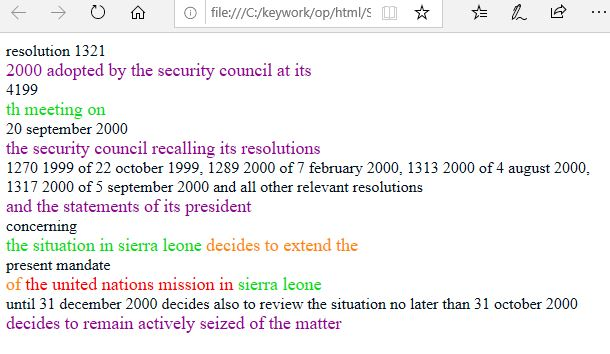
\includegraphics[width=\textwidth]{figures/forsyth-img001.jpg}
\caption{Text of UN Security Council resolution 1321, colour-coded by flicshow}
\label{fig:forsyth:1}
\end{figure}

\begin{table}
\caption{Colour-coding by longest $n$-gram that covers a particular token (default mode)\label{tab:forsyth:5}}
\begin{tabular}{ll}
\lsptoprule
Score & Colour\\\midrule
6+ & purple\\
5 & red\\
4 & orange\\
3 & green\\
2 & blue\\
1 & cyan\\
0 & black\\
\lspbottomrule
\end{tabular}
\end{table}


The format here is that each change from covered to uncovered text corresponds to a new line, so the original layout is lost; moreover, punctuation has been ignored, as in previous examples. The last line, \textit{decides to remain actively seized of the matter}, is an 8-gram. As already mentioned, the system was using up to 6-grams, so this indicates how fragmented portions of a sequence can overlap to give a better idea of the natural length of a repeated sequence.

More interesting is the third line from the bottom, \textit{of the united nations mission in sierra leone}. This begins with a single token \textit{of} in orange. Orange is the colour of 4-grams, but each token gets the colour of the longest $n$-gram that covers it; so this implies that the 4-gram \textit{of the united nations} was, in a sense, trumped by the 5-gram \textit{the united nations mission in}. Similarly, the last two words, \textit{sierra leone} are in green, indicating a 3-gram, but presumably the 3-gram \textit{in sierra leone} is also trumped by the same 5-gram, so that its leading token, \textit{in}, receives the colour of the longer sequence, in which it is the final token.

The intent of this colour scheme is to assist investigation of phraseological patterns by highlighting what might be termed a quasi-syntax, showing how longer collocades are built up from shorter segments. \figref{fig:forsyth:2} shows another example, from the Hong Kong Tripadvisor postings, one that received many replies.

  

\begin{figure}[p]
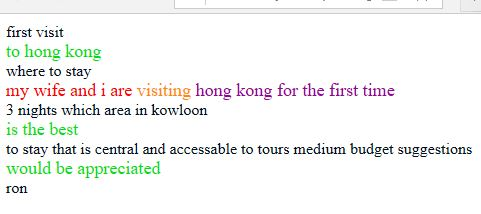
\includegraphics[width=.9\textwidth]{figures/forsyth-img002.jpg}
\caption{Colour-coded collocades in HK Tripadvisor forum posting}
\label{fig:forsyth:2}
\end{figure}



\begin{figure}[p]
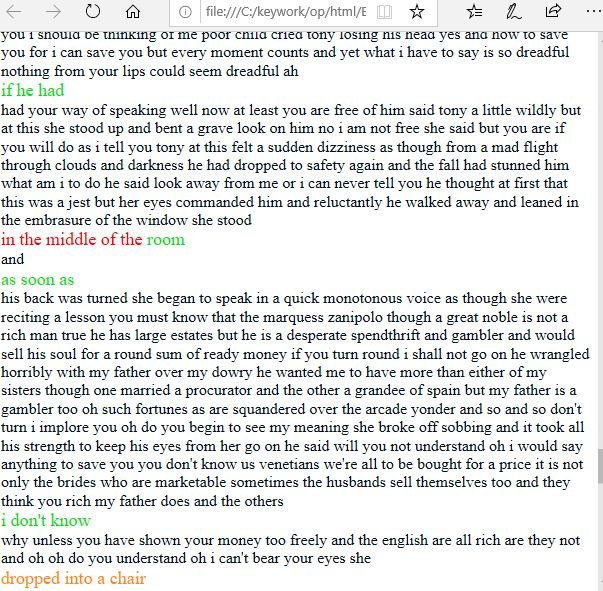
\includegraphics[width=.9\textwidth]{figures/forsyth-img003.jpg}
\caption{Extract from a tale by Edith Wharton}
\label{fig:forsyth:3}
\end{figure}

By contrast, \figref{fig:forsyth:3} shows output from flicshow when applied to a story by Edith Wharton called Venetian Nights. This extract exhibits long blocks of running text in black, with only a scattering of highlighted $n$-grams, most of which do not connect or overlap.

\section{Classification via collocade coverage}\label{sec:forsyth:6}

The taverns program (Textual Affinity Values Employing Repeated N-gram Sequences) uses the formulexicon in a slightly different way, intended to indicate which texts are typical and atypical of their category and indicate how distinctive the categories are among themselves.

Inspecting individual texts can be a valuable opportunity to get close to the data, but in a typical corpus there is a huge amount of data to be inspected. The program taverns works in bulk mode and thereby gives an indication of which particular files might deserve the kind of close attention given to the output of flicshow. It goes a step further than formulex, using the same method, by computing coverage of each text specified not only by the $n$-grams of its own category, but by those of all the categories in the formulexicon file. Thus, in effect, it ranks each text file according to how typical it is of each category, including its own. Normally these texts are an unseen holdout sample, not used by outgrams to create the formulexicon.

In addition, having done this, it performs text classification by assigning each text to the category which gives it the highest coverage score. It is not intended primarily as a text classifier, but the results in classification mode often shed light on the relationships between the text types involved, as well as identifying typical and anomalous texts.

The listing below shows the first 15 and last 15 lines of the taverns output for coverage by the BEER formulexicon.\bigskip

\begin{lstlisting}[basicstyle=\small\ttfamily]
Ranking by coverage of sequences from beer

   1    587    97   47.53  47.42  beer     youngs_hummingbird.txt
   2    586   100   44.37  43.00  beer     sol_cerveza.txt
   3    438    79   42.01  40.51  beer     budweiser.txt
   4    651   111   41.47  40.54  beer     tolly_english_ale.txt
   5    595   100   41.01  41.00  beer     wells_bombardier.txt
   6    636   105   35.69  36.19  beer     lancaster_blonde.txt
   7    709   123   34.41  33.33  beer     mcewans_amber.txt
   8    568    90   33.98  34.44  beer     marstons_burton_bitter.txt
   9    808   135   32.18  28.89  beer     blacksheep_venusmars.txt
  10   1101   186   31.06  29.57  beer     spitfire.txt
  11    683   120   29.28  28.33  beer     brains_sa.txt
  12    592   102   28.89  29.41  beer     wadworth_ipa.txt
  13    561    96   26.92  27.08  beer     yorkshire_gold.txt
  14    931   153   26.85  26.80  beer     weetwood_southern\_cross.txt
  15    571    92   26.27  27.17  wine     domaine_mandeville.txt

[.... many lines omitted ....]

 676   7397  1287    0.00   0.00  leaflet  Angitil_SR.txt
 677   5045   909    0.00   0.00  leaflet  Amoxil_Syrup.txt
 678   4384   789    0.00   0.00  leaflet  Amoxil_Capsules.txt
 679   6619  1144    0.00   0.00  leaflet  Algitec_Chewtab_Tablets.txt
 680   6198   946    0.00   0.00  leaflet  Adenocor.txt
 681  12823  2238    0.00   0.00  leaflet  Actrapid_Pen.txt
 682    762   123    0.00   0.00  wine     two_oceans_chardonnay.txt
 683   1072   180    0.00   0.00  wine     rina_ianca.txt
 684    483    75    0.00   0.00  wine     perlage_pinot_grigio.txt
 685    638   111    0.00   0.00  wine     paulmas_vinus.txt
 686    812   139    0.00   0.00  wine     la_chiave_2013.txt
 687    569    92    0.00   0.00  wine     finca_fabian.txt
 688    972   153    0.00   0.00  wine     era_puglia_falanghina.txt
 689    649   105    0.00   0.00  wine     domaine_begude.txt
 690    532    92    0.00   0.00  wine     doblez_garnacha.txt
\end{lstlisting}

The first item refers to the text of the back label of Young's Hummingbird ale. The first number is its rank, 1. The next two numbers give its size in characters and tokens, 587 and 97. The next two numbers show that 47.53\% of its characters and 47.42\% of its tokens were covered by 3- to 6-grams from the formulexicon of the BEER category. The last two columns give the actual category of the text and its file name. Note that this is a genuine holdout test, on 690 files that were not used by outgrams to create the formulexicon.

It will be seen that one WINE text creeps into the top 15 items as measured by typicality to the BEER category. In the bottom 15 items there are nine WINE texts. However, only 117 texts have more than zero coverage by the BEER formulexicon, so the order of the last 573 texts, with no coverage at all, is essentially arbitrary.

After listing each text as covered by $n$-grams from the formulexicon of each category (7 in this case) the program classifies each text according to how much of it is covered by each category's $n$-grams, taking maximum coverage to decide the assigned category. For the present example, the most confident 15 entries are listed below.\bigskip

\begin{lstlisting}[basicstyle=\small\ttfamily]
Results in classification mode:

      relative   actual       categories
rank  coverage% coverage%     pred : true      docname
   1    100.00    35.29       sres + sres  S_RES_12942000-en.txt
   2    100.00    30.10       sres + sres  S_RES_13362001-en.txt
   3    100.00    30.09       sres + sres  S_RES_15002003-en.txt
   4    100.00    29.86       sres + sres  S_RES_13162000-en.txt
   5    100.00    29.85       sres + sres  S_RES_14762003-en.txt
   6    100.00    29.63       sres + sres  S_RES_14432002-en.txt
   7    100.00    28.53       sres + sres  S_RES_13482001-en.txt
   8    100.00    27.94       sres + sres  S_RES_13882002-en.txt
   9    100.00    24.90       sres + sres  S_RES_14582003-en.txt
  10    100.00    24.86       sres + sres  S_RES_15182003-en.txt
  11    100.00    24.73       sres + sres  S_RES_14652003-en.txt
  12    100.00    24.10       sres + sres  S_RES_15482004-en.txt
  13    100.00    24.03       sres + sres  S_RES_13872002-en.txt
  14    100.00    23.73    leaflet + leaflet  SlowFe.txt
  15    100.00    23.62       sres + sres  S_RES_15302004-en.txt

\end{lstlisting}

The top line of this output signifies that Security Council resolution 1294 (from year 2000) has 35.29\% coverage by SRES $n$-grams. The number in the second column, 100.00, indicates that this 35.29\% represents 100\% of the total coverage by all seven formulexicons, i.e., that $n$-grams from no category apart from SRES covered any of this text. These are the most confident classifications, 14 of the 15 being Security Council resolutions and one a medicine information leaflet.

The column labels ``pred'' and ``true'' stand for predicted and true category. The segment ``sres + sres'' means that this file was predicted to belong to the SRES class and it was indeed from that class. The plus sign marks a correct decision: a minus sign would appear if it were incorrect and a question mark if the text's category were unknown.

Overall classification performance is summarized at the foot of the output listing by a confusion matrix, such as that for the present example, listed below.
\medskip

\begin{lstlisting}[basicstyle=\small\ttfamily]
Confusion matrix:

Truecat =          EW     beer  fewreps  leaflet manyreps  sres  wine
Predcat : EW       23        0        3        0        6    0      0
Predcat : beer      0       37        0        0        0    0      4
Predcat : fewreps   0        0       10        1       42    0      0
Predcat : leaflet   0        0        0      172        1    0      0
Predcat : manyreps  0        0       65        0      189    0      2
Predcat : sres      0        0        1        0        0  100      0
Predcat : wine      0        0        0        0        0    0     34
\end{lstlisting}


% \begin{figure}
% 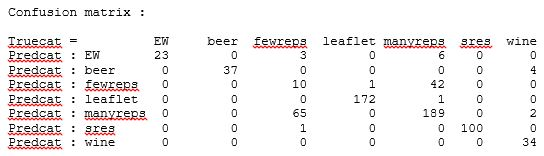
\includegraphics[width=\textwidth]{figures/forsyth-img004.jpg}
% \end{figure}
%
% \begin{table}
% \resizebox{\textwidth}{!}{\begin{tabular}{lrrrrrrr}
% \lsptoprule
% Truecat =          & EW  &   beer & fewreps & leaflet & manyreps &  sres & wine\\\midrule
% Predcat : EW       & 23  &      0 &       3 &       0 &        6 &    0  &    0\\
% Predcat : beer     &  0  &     37 &       0 &       0 &        0 &    0  &    4\\
% Predcat : fewreps  &  0  &      0 &      10 &       1 &       42 &    0  &    0\\
% Predcat : leaflet  &  0  &      0 &       0 &     172 &        1 &    0  &    0\\
% Predcat : manyreps &  0  &      0 &      65 &       0 &      189 &    0  &    2\\
% Predcat : sres     &  0  &      0 &       1 &       0 &        0 &  100  &    0\\
% Predcat : wine     &  0  &      0 &       0 &       0 &        0 &    0  &   34\\
% \lspbottomrule
% \end{tabular}}
% \caption{[As a Table.]}
% \end{table}

Here the procedure makes 125 errors out of 690 decisions, about 18\%, but only 18 of these mistakes, 2.6\% of all 690 cases, arise from categories other than FEWREPS and MANYREPS. Essentially, this means that the system cannot distinguish between Hong Kong forum posts that receive few replies and those that receive many. Given how short these texts are (median sizes of 56 and 80 tokens) it would have been surprising, though interesting, if the two classes had been readily distinguishable by such a process. On the other hand, the other categories, even BEER and WINE, are well distinguished on this basis.
\newpage

To give a point of comparison, the method described in \citet{Wright2017} was implemented and applied to the same dataset. Wright obtained good results with this method in classifying messages from the Enron email corpus \citep{Cohen2009}, according to the author. Each text was assigned the category with the highest similarity score based on the Jaccard coefficient (J) using sets of $n$-grams. The Jaccard coefficient divides the size of the set intersection by the size of the set union as in the formula

\ea
  J = {\textbar}A ${\cap}$ B{\textbar} / {\textbar}A ${\cup}$ B{\textbar}
\z
where A is the set of $n$-grams in a single test text and B is the set of $n$-grams in the group of texts belonging to a particular category.

Wright's best results were found with tetragrams (4-grams) so that 4-grams were used on the same data as processed by the taverns program, above. Where taverns achieved a classification success rate of 81.88\% (565/690), the Jaccard-similarity technique achieved 79.71\% (550/690). When ignoring cases with zero similarity to any category, the rates were 83.77\% (542/647) with taverns and 81.39\% (503/618) with Jaccard similarity. This is only a single data point, but it does suggest that the present approach of using $n$-gram coverage gives results that are competitive with an established technique for this sort of application.

\section{Clues from clusters of collocades}\label{sec:forsyth:7}

The previous sections have concentrated on analyses of individual texts or text categories; but a researcher in this field will typically not only be interested in how formulaic particular texts are, how typical or atypical they are of their class, and how similar or different a group of text types are amongst themselves, but also on how the repetitive sequences identified in this process relate to each other. In other words, it would be desirable for researchers into formulaic language to have a tool that helps to shed light on the patterns of phraseology that are responsible for high or low scores in terms of collocade coverage.

The program postflab is designed with this aim in mind. It uses a secondary output file of formulex, the flab listing (Frequently Assembled Lexical Bundles) as input and attempts to organize these frequent collocades in a manner that brings out their interrelationships.

An extract from a flab output file follows to illustrate the kind of data in question. This specimen consists of the first twelve lines from the patient information leaflet subcorpus.\bigskip

\begin{lstlisting}
3 leaflet 288 294415 1689519
 0.2868   285   16   3  tell your doctor
 0.2294   323   11   3  if you have
 0.2162   332   10   3  if you are
 0.1951   206   15   3  your doctor may
 0.1932   192   16   3  your doctor will
 0.1888   145   21   3  the active ingredient
 0.1749   197   14   3  you are taking
 0.1715   138   20   3  taking your medicine
 0.1545    30   86  16  if you have any questions or are not sure about anything ask your doctor or pharmacist
 0.1509    85   29   5  ask your doctor or pharmacist
 0.1442    84   28   6  out of the reach of children
 0.1406   198   11   3  do not take
\end{lstlisting}

The first line merely identifies the text category, and adds the information that it contains 288 files, comprising 294,415 tokens and 1,689,519 characters.

The next line shows that the collocade which covers the largest proportion of the subcorpus overall is ``tell your doctor''. This contains three tokens, is 16 characters in length and occurs 285 times altogether in that text category. The figure 0.2868 is a percentage, the percentage of the entire text of the subcorpus that is covered by this 3-token sequence. Further down the list, we can see the longest of these collocades ``if you have any questions or are not sure about anything ask your doctor or pharmacist'', a 16-element collocade that contains 86 characters and covers 0.1545\% of the whole subcorpus, occurring 30 times.

A proportion of 0.1545\% may seem tiny, but given that the commonplace triple ``one of the'' is the most frequent collocade in the tales by Edith Wharton, covering a mere 0.0692\% of the EW subcorpus, a 16-token sequence that accounts for even 0.1545\% of a text corpus is worthy of attention.

A point to realize about such listings is that each item coverage is computed separately. For example, the eleventh item, ``ask your doctor or pharmacist'', occurring 85 times, is a substring of the item immediately preceding it. What this implies is that the shorter string occurs $30+85 = 115$ times altogether. It occurs 30 times preceded by ``if you have any questions or are not sure about anything'' and 85 times without that preceding context. This avoids double counting.

The principle behind this mode of reckoning coverage can best be explained with reference to the bigram \textit{your doctor}. This pair of tokens forms part of the items \textit{tell your doctor}, \textit{your doctor may} and \textit{your doctor will}, as well as the two longer items just discussed. As it happens, that particular word-pair occurs 2193 times in this training sample. What the figure of 206 next to \textit{your doctor may} tells us is that of these 2193 occurrences, 206 are followed immediately by \textit{may}; and likewise with the other collocades containing \textit{your doctor}.

The finding that shorter sequences often occur within longer collocades hints at a kind of network of phraseological possibilities surrounding a core component. However, because the flab output is listed in frequency order, it is very tedious to extract such information from the data as given. The program postflab is intended to alleviate this problem.

This program reads in the flab output produced by formulex and performs a 1-dimensional scaling on the collocades concerned, using string similarity as the value to be optimized. Multidimensional scaling \citep{UptonCook2006}  is a statistical optimization procedure which aims to reproduce as closely as possible a matrix of distances between items by assigning to each item coordinate values on a small number of dimensions. In the present case, rather unusually, the algorithm is applied with just a single dimension. In the postflab program, the process is taken to its minimal form, which means that the items are arranged in a single linear order that tries as far as possible to ensure that distances along the line correlate with distances derived from the entire matrix of inter-item similarities. In effect, the procedure adds, for strings, the concept of similarity order to the well-known concepts of alphabetic order and frequency order.

The derived ordering is written to a text file for inspection and also, more usefully, to a data file to be processed in R so that it can be displayed visually. \figref{fig:forsyth:4} shows the results of this procedure for the 36 most frequent collocades from the medical leaflet category.

  
\begin{figure}
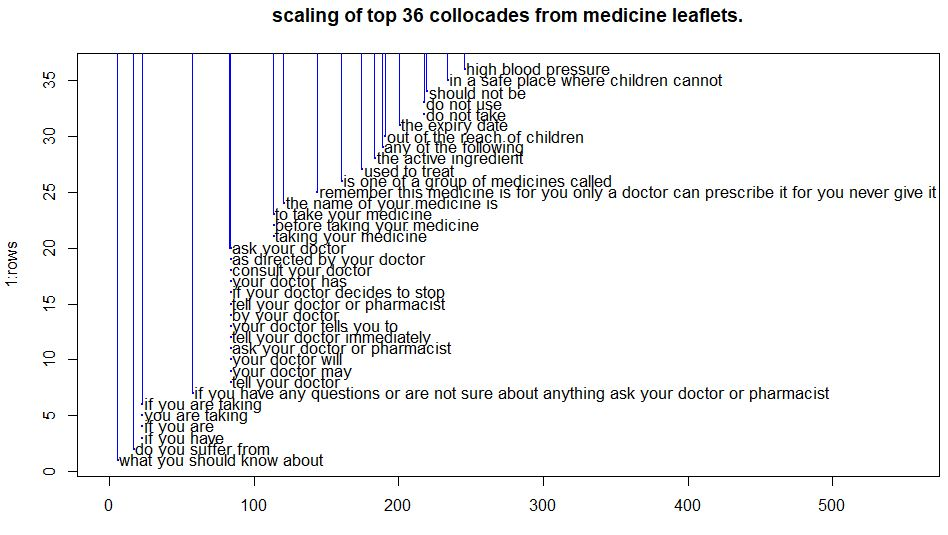
\includegraphics[width=\textwidth]{figures/forsyth-img005.jpg}
\caption{One-dimensional scaling of collocades from medical leaflet category}
\label{fig:forsyth:4}
\end{figure}

In this diagram the vertical axis merely separates the items so that they do not overwrite each other. The horizontal axis represents the closeness of the items along a single dimension. The width of the blue lines is proportional to the aggregate coverage of all the collocades with the same score on the x-axis. These lines are intended to reveal the presence of certain groupings along the x-axis, including the main grouping which consists of a number of collocades containing the digram ``your doctor''. Hence the program has performed a clustering as a side-effect.

Although this graphic representation is based only on superficial string similarity, and has no semantic underpinning, it nevertheless makes it much easier for a researcher to find clusters of related phrasings than the text-based listing.

\section{Concluding remarks}\label{sec:forsyth:8}
\largerpage
The formulib package implements one particular way of operationalizing the concept of formulaic language by using a traditional resource, the frequent $n$-gram list, in a slightly novel manner. It constitutes an innovative tool based on a simple idea, which offers the researcher informative ways of viewing repetitive phrasings in a corpus or collection of corpora. It takes further the work of \citet{ForsythGrabowski2015} by providing estimates of how much formulaic language is found in individual texts as well as how formulaic certain text types are. Although the examples quoted in the present chapter are in English, formulib can be applied to any language, and it does not need pre-processing resources such as lexicons, parsers or taggers.

We cannot expect a single approach to cover all the different aspects of such a complex phenomenon as formulaic language. However, the argument of this chapter is that the concept that underlies the methods employed by the formulib software, namely collocade coverage, offers a straightforward and relatively effective way of investigating some of the more important aspects of formulaic language.

Formulib cannot, of course, be regarded as an endpoint in the continuing attempt to explore patterns of formulaic sequences. Even staying with collocade coverage as a key indicator, there is room for further development. For instance, it would be highly desirable to find a more precise notation for integrating clearly related elements of the formulexicon such as

\begin{quote}
\textit{please read this leaflet carefully before taking your tablets}
\end{quote}
and

\begin{quote}
\textit{please read this leaflet carefully before you take your medicine}
\end{quote}
into a form that reveals their relatedness (a kind of micro-grammar). The two items above could be unified with the aid of a pattern-description language, such as the following.

\begin{quote}
\textit{please read this leaflet carefully before} [\textit{taking} {\textbar} \textit{you take}] \textit{your} [\textit{medicine} {\textbar} \textit{tablets}]
\end{quote}

However, to do this efficiently and reliably would require leading-edge artificial intelligence applied to the induction of a small-scale grammar, and the results would doubtless be hard to interpret without advanced data visualization techniques. Perhaps a reader may take up that challenge. At any rate, the present chapter shows this approach opens up plenty of avenues for further research.

\largerpage
{\sloppy\printbibliography[heading=subbibliography,notkeyword=this]}
\end{document}
